\documentclass[12pt]{article} % 12pt 为字号大小 UTF8
\usepackage{amssymb,amsfonts,amsmath,amsthm}
%\usepackage{fontspec,xltxtra,xunicode}
%\usepackage{times}

%----------
% 定义中文环境
%----------

\usepackage{xeCJK}

% \setCJKmainfont[BoldFont={SimHei},ItalicFont={KaiTi}]{SimSun}
% \setCJKsansfont{SimHei}
% \setCJKfamilyfont{zhsong}{SimSun}
% \setCJKfamilyfont{zhhei}{SimHei}

% \newcommand*{\songti}{\CJKfamily{zhsong}} % 宋体
% \newcommand*{\heiti}{\CJKfamily{zhhei}}   % 黑体


%----------
% 版面设置
%----------
%首段缩进
\usepackage{indentfirst}
\setlength{\parindent}{2.1em}

%行距
\renewcommand{\baselinestretch}{1.4} % 1.4倍行距

%页边距
\usepackage[a4paper]{geometry}
\geometry{verbose,
	tmargin=3cm,% 上边距
	bmargin=3cm,% 下边距
	lmargin=3cm,% 左边距
	rmargin=3cm % 右边距
}


%----------
% 其他宏包
\usepackage{listings}

%----------
%图形相关
\usepackage[x11names]{xcolor} % must before tikz, x11names defines RoyalBlue3
\usepackage{graphicx}
\usepackage{pstricks,pst-plot,pst-eps}
\usepackage{subfig}
\def\pgfsysdriver{pgfsys-dvipdfmx.def} % put before tikz
\usepackage{tikz}

%原文照排
\usepackage{verbatim}

%网址
\usepackage{url}
\usepackage[framed,numbered,autolinebreaks,useliterate]{mcode}

%----------
% 习题与解答环境
%----------
% %习题环境
% \theoremstyle{definition} 
% \newtheorem{exs}{习题}

% %解答环境
% \ifx\proof\undefined\
% \newenvironment{proof}[1][\protect\proofname]{\par
% \normalfont\topsep6\p@\@plus6\p@\relax
% \trivlist
% \itemindent\parindent
% \item[\hskip\labelsep
% \scshape
% #1]\ignorespaces
% }{%
% \endtrivlist\@endpefalse
% }
% \fi

% \renewcommand{\proofname}{\it{证明}}

%----------
% 我的自定义
%----------

\newcommand{\horrule}[1]{\rule[0.5ex]{\linewidth}{#1}} 	% Horizontal rule

\renewcommand{\refname}{参考文献}
\renewcommand{\abstractname}{\large \bf 摘\quad 要}
\renewcommand{\contentsname}{目录}
\renewcommand{\tablename}{表}
\renewcommand{\figurename}{图}

\setlength{\parskip}{0.4ex} % 段落间距

\usepackage{enumitem}
\setenumerate[1]{itemsep=0pt,partopsep=0pt,parsep=\parskip,topsep=5pt}
\setitemize[1]{itemsep=0.4ex,partopsep=0.4ex,parsep=\parskip,topsep=0.4ex}
\setdescription{itemsep=0pt,partopsep=0pt,parsep=\parskip,topsep=5pt}


%==========
% 正文部分
%==========

\begin{document}
	
	\title{
		%	{\normalfont\normalsize\textsc{
		%			Xiangtan University  \\[25pt]}}
		\horrule{0.5pt}\\
		\sffamily{数值计算方法实验报告\\不动点迭代法与牛顿迭代法}
		\horrule{1.8pt}\\[20pt]
	}
	\author{米科润\quad 19信计二班\\201905755824}
	\date{\today} % 若不需要自动插入日期,则去掉前面的注释;{ } 中也可以自定义日期格式
	
	\begin{titlepage}
		\maketitle
		\vspace{30pt}
		\thispagestyle{empty}
	\end{titlepage}
	
	\tableofcontents
	\thispagestyle{empty}
	
	\newpage
	\setcounter{page}{1}
	
	\section{实验题目}
	\indent 1、生成一个系数由(0,7)之间的随机数组成的七次多项式,并使用不多点迭代法和牛顿迭代法找出解、收敛阶、收敛速度。\\
	\indent 2、将$x^2+(\frac{5}{4}\times y- \sqrt(\left| x\right|))^2-4=0$的图像画出来。
	
	\section{实现算法}
	书本217至227的算法
	
	
	
	\section{程序代码}
	不动点迭代法代码:Fixed Point Iteration.m
	\begin{lstlisting}
		function []=F_P_Iteration(f,x0)
		%%
		%初始设置
		syms x
		f(x)=f;
		m=20;TOL=1e-6;
		df(x)=diff(f(x));
		a=-100;b=100;
		phi=df(a:0.05:b);
		x1=x0;
		t=0;
		%%
		%判断是否收敛
		if  abs(double(phi)) <= 1
			disp('具有全局收敛性');
		end
		%%
		%迭代
		for i=1:m
			xx=f(x1);
			if abs(double(xx)-double(x1))<=TOL
				disp('迭代次数为:');
				disp(i);
				t=1;
				break;
			end
			x1=double(xx);
		end
		if t==1
			disp('不动点为:');
			disp(double(xx));
		else
			warning('未迭代到解');
		end
		%%
		%判断收敛阶
		if t==1
			c=zeros(1,7);
			for j = 1:7
				delta(x)=diff(f,j);
				c(j)=double(delta(xx));
			end
			I1=find(c,1,'first');
			disp('收敛阶为:');
			disp(I1);
		end
		end
	\end{lstlisting}
	\indent 牛顿迭代法代码:Newton Iteration.m
	\begin{lstlisting}
		function []=Newton_Iteration(f,x0)
		%%
		syms x 
		f(x)=f;
		m=20;TOL=1e-6;
		a=-2;b=2;
		dy(x)=diff(f(x));
		ddy=dy(a:0.05:b);
		x1=x0;
		t=0;
		%%
		if (double(f(a))*double(f(b))<0) & (double(ddy)~=0) & (abs(double(f(a))/double(dy(a)))<(b-a)) ...
		& (abs(double(f(b))/double(dy(b)))<(b-a))
			disp('迭代收敛唯一解,收敛阶数为2');
		end
		%%
		for i=1:m
			xx=f(x1);
			if abs(double(xx)-double(x1))<=TOL
				disp('迭代次数为:');
				disp(i);
				t=1;
				break;
			end
			x1=double(xx);
		end
		if t==1
			disp('解为:');
			disp(double(xx));
		else
			warning('未迭代到解');
		end
		end
	\end{lstlisting}
	\indent 运行代码:test iteration.m
	\begin{lstlisting}
clc,clear
A=7*rand(8,1);
syms x
f=A(7)*x^7+A(6)*x^6+A(5)*x^5+A(4)*x^4+A(3)*x^3+A(2)*x^2+A(1)*x+A(8);
x0=0.5;
disp('不动点迭代结果:');
for k = 1:7
	g=(f-x^k)^(1/k);
	F_P_Iteration(g,x0);
end
%F_P_Iteration(f,x0);
f=x-f/diff(f);
disp('牛顿迭代法迭代序列为:');
pretty(f);
disp('牛顿迭代结果:');
Newton_Iteration(f,x0);
syms x y 
F=x.^2+(5/4.*y-sqrt(abs(x))).^2-4; 
fimplicit(F,[-3,3 -3,3])
	\end{lstlisting}
	\section{实验结果}
	运行test Iteration.m
	\indent 可得运算结果:
	\begin{figure}[ht]
		\centering
		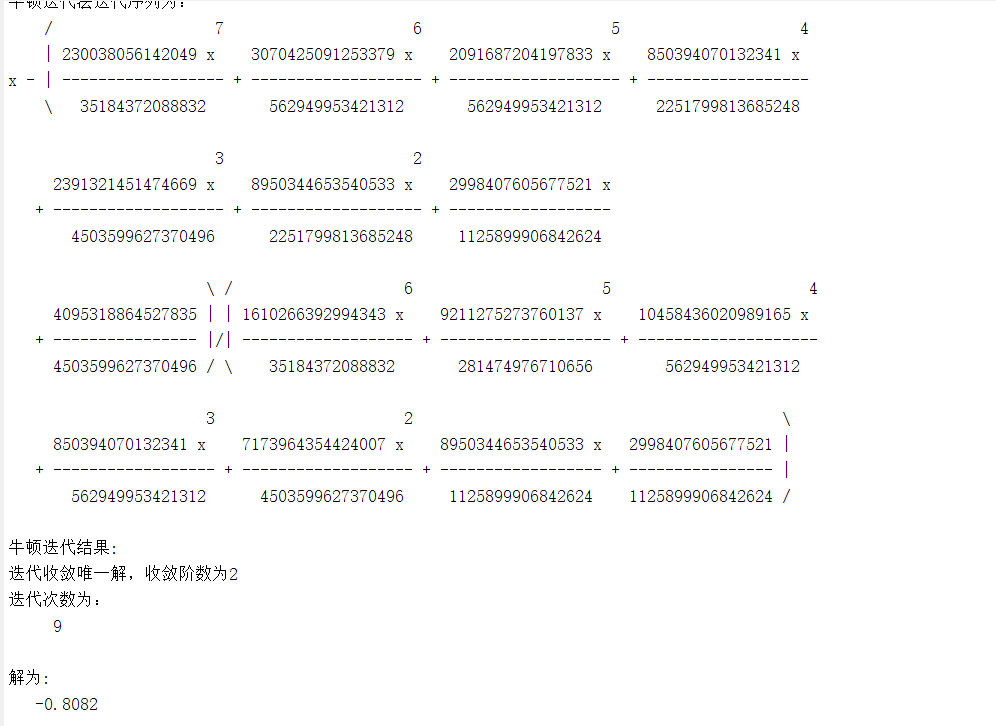
\includegraphics[width=0.8\textwidth]{Iteration.png}
		\caption{result1}
		\label{fig:fig1}
		\centering
	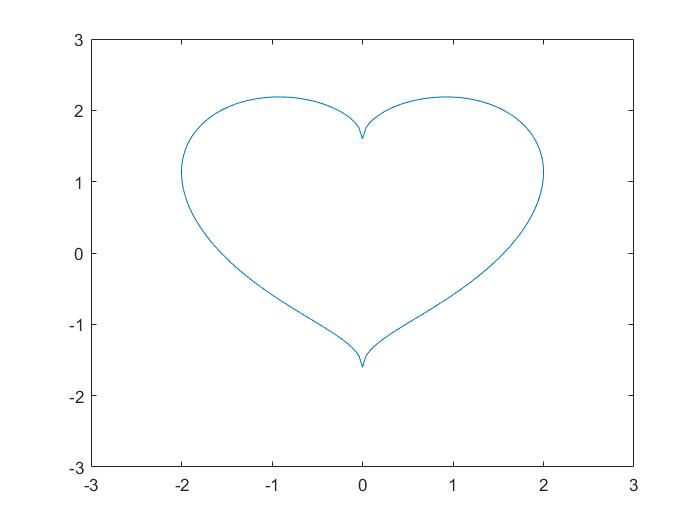
\includegraphics[width=0.8\textwidth]{figure.jpg}
	\caption{result2}
	\label{fig:fig1}		
	\end{figure}
	% \section{习题环境}
	
	% \begin{exs}
	% 请证明勾股定理。
	% \end{exs}
	% \begin{proof}
	% 这是证明。末尾后会自动添加方块以示结束。
	% \end{proof}
	
	% \begin{exs}
	% 请计算 $1+2+\ldots +100$。
	% \end{exs}
	% \begin{proof}[解答]
	% 这是解答。末尾后会自动添加方块以示结束。
	% \end{proof}
	
	
\end{document}